%%%%%%%%%%%%%%%%%%%%%%%%%%%%%%%%%%%%%%%%%%%%%%%%%%%%%%%%%%%%%%%%%%%%%%%%%
% Abgabe:    17. Dezember 2018 bis 20.00 Uhr  
% Dateiname: 181217 Mustermann Max Facharbeit 
% Wer alle Hausaufgaben gemacht hat, kopiert nur
% aus den korrigierten Texten und fügt entsprechend ein.
% Tipp: benutze Strg+c zum Kopieren von Texten
%       und     Strg+v zum Einfügen von Texten
% Bitte die aktuellen Zeilennummer benutzen!!
%%%%%%%%%%%%%%%%%%%%%%%%%%%%%%%%%%%%%%%%%%%%%%%%%%%%%%%%%%%%%%%%%%%%%%%%%
% Hier nichts verändern!
\documentclass[12pt,a4paper]{scrartcl}  
\usepackage[utf8]{inputenc}
\usepackage[ngerman]{babel}
\usepackage{geometry} 
\usepackage{graphicx} 
\usepackage{float}
\usepackage{wrapfig} 
\usepackage{verse}
\usepackage{lineno}
\sloppy
\linespread{1.4} 
\setlength\parindent{0pt} 
%------------------------------------------------
\begin{document}
% Titelseite: Hier nichts verändern!
\begin{titlepage}
\newcommand{\HRule}{\rule{\linewidth}{0.5mm}} 
\center 
\textsc{\LARGE Europaschule Langerwehe}\\[1.5cm] 
\textsc{\Large Facharbeit Deutsch}\\[0.5cm] 
\textsc{\large 10 E-Kurs}\\[0.5cm] 
\HRule \\[0.8cm]
{ \huge \bfseries Satire}\\[0.4cm] 
\HRule \\[1.5cm]
\begin{minipage}{0.4\textwidth}
\begin{flushleft} \large
\emph{Autor:}\\
Max \textsc{Mustermann} % Deinen Namen einsetzen
\end{flushleft}
\end{minipage}
~
\begin{minipage}{0.4\textwidth}
\begin{flushright} \large
\emph{Lehrer:} \\
Herr \textsc{Fischer}
\end{flushright}
\end{minipage}\\[4cm]
{\large \today}\\[3cm] 
\vfill 
\end{titlepage}
%------------------------------------------------
% Inhaltsverzeichnis. Bitte nichts ändern!
\tableofcontents 
\newpage 
%------------------------------------------------
% Dank an Simon für die Digitalisierung der Karikatur.
%
\begin{figure}[H] % Zirkus.jpg muss im Verzeichnis sein!
\center{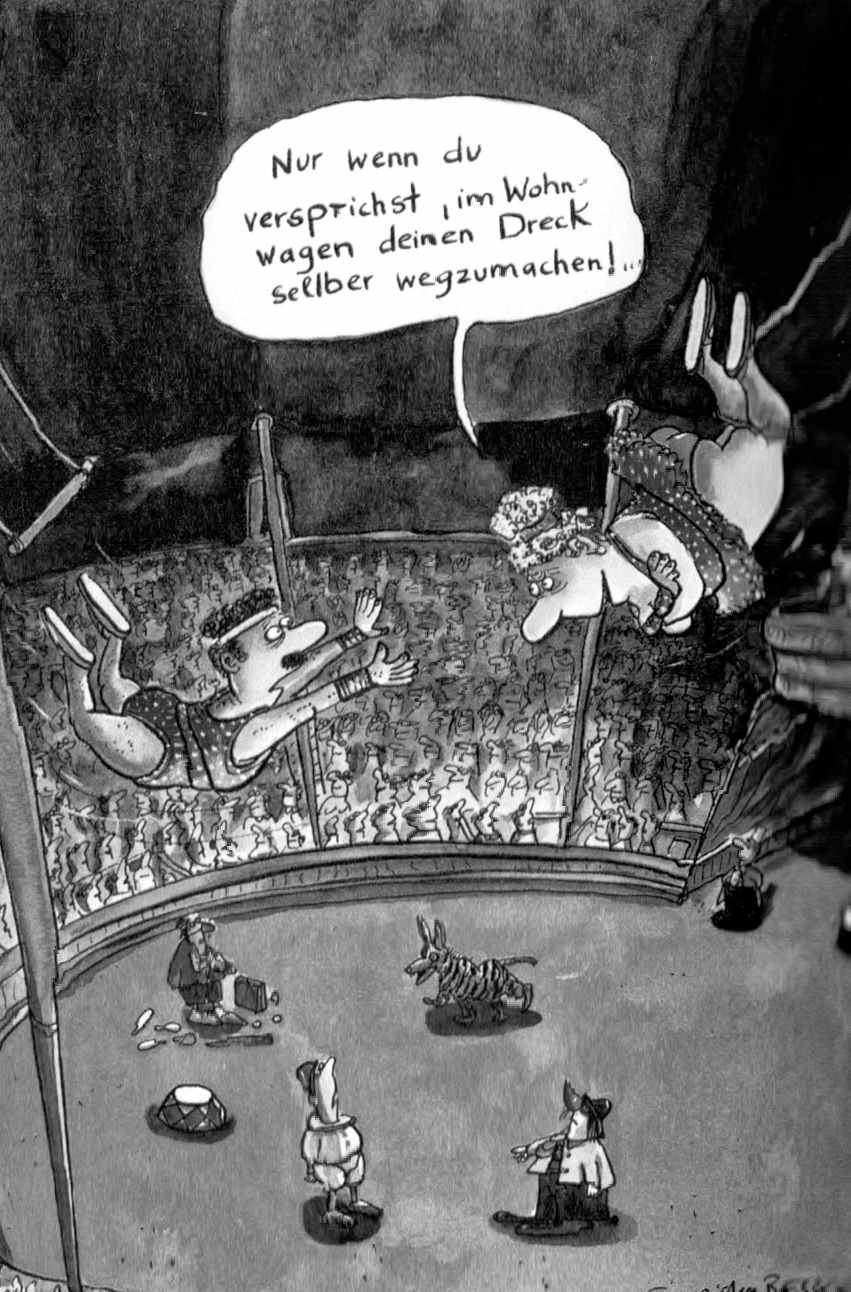
\includegraphics[width=0.5\linewidth]{Zirkus.jpg}}
\caption{Zirkus (S.209)}
\label{fig:speciation}
\end{figure}
%------------------------------------------------
\section{Eine Karikatur analysieren}
% Hier geht's los mit der 1. Hausaufgabe:
PLATZHALTER


%------------------------------------------------
% Dank an Simon, der den Text formatiert hat.
%------------------------------------------------
\section{Einen Liedtext untersuchen} 
 \newcommand{\attrib}[1]{\nopagebreak{\raggedleft\footnotesize #1\par}}
  \subsection*{Frauen kommen langsam, aber gewaltig}
 \settowidth{\versewidth}{Männer sind auf dieser Welt einfach unersetzlich.;}
 \poemlines{4}

 \begin{verse}[\versewidth]
Schlaue Frauen sind verdächtig\\
nehmen alles in die Hand\\
schlaue Frauen beweisen\\
täglich ihr'n Verstand\\
schlaue Freuen schlag'n auf'n Magen\\
müssen immer besser sein\\
schlaue Frauen jagen\\
Männern Ängste ein\\!

Frauen machen ständig klar\\
Frauen lieb'n sich sonderbar\\
Frauen setzen alles dran\\
Frauen nehm'n es wie'n Mann\\!

\textbf{Chorus:}\\
Starker Mann was nun\\
keine Zeit mehr was zu tun\\
Frauen kommen langsam\\
- aber gewaltig\\!

Starke Frauen hab'n schwache Nerven\\
müssen wie ein Wunder sein\\
starke Frauen trinken\\
heimlich ganz allein\\
starke Frauen sind wie Kinder\\
wollen Komplimente hör'n\\
starke Frauen lassen\\
sich schnell irreführ'n\\!

Frauen sind wie im Roman\\
rufen immer zuerst an\\
Frauen suchen Zärtlichkeit\\
wollen was auf Ewigkeit\\!

\textbf{Chorus:}\\
Starker Mann was nun\\
keine Zeit mehr was zu tun\\
Frauen kommen langsam\\
- aber gewaltig\\!

Frauen gibt man immer Küsse\\
hassen ihre Kompromisse\\
Frauen hab'n Schlankheitstick\\
finden sich immer zu dick\\
Frauen macht die Liebe blind\\
wünschen sich heimlich 'n Kind\\
Frauen frag'n sich immer was\\
kriegen ohne Männer Spaß\\!

\textbf{Chorus:}\\
Starker Mann was nun\\
keine Zeit mehr was zu tun\\
Frauen kommen langsam\\
- aber gewaltig\\!


Schöne Frauen hab's leichter\\
hab'n die alten Trickse drauf\\
schone Frauen fängst man\\
vor dem Fallen auf\\
schöne Frauen werd'n blöd angequatscht\\
und billig angemacht\\
schöne Frauen muß man\\
'rumkrieg'n für 'ne Nacht\\!

\textbf{Chorus:}\\
Starker Mann was nun\\
keine Zeit mehr was zu tun\\
Frauen kommen langsam\\
- aber gewaltig\\!

 \end{verse}
  % Nennung des Autoren:
 \attrib{Ina Deter 1986}
%------------------------------------------------
\subsection{Das Lied} 
% Hier geht's los mit der 2. Hausaufgabe:
PLATZHALTER

%------------------------------------------------
\subsection{Allgemeine Informationen} 
PLATZHALTER



%------------------------------------------------
\subsection{Die Frauentypen und die Reaktionen der Männer} 
PLATZHALTER

%------------------------------------------------
\subsection{Sprachliche Analyse}
PLATZHALTER


%------------------------------------------------
\subsection{Eigene Stellungnahme} 
PLATZHALTER


%------------------------------------------------
\section{Einen Prosatext untersuchen}
\modulolinenumbers[5]
\begin{linenumbers}
\subsection*{Handtaschenfabrikverkauf in Nussloch}
Du kannst in einer Fabrik einkaufen. Das wusste ich nicht. Frauen fahren in die Fabrik, die fahren in die Fabrik rein. Die fahrn rein in die Fabrik. Das wird vom Band weggenommen, das wird nicht mehr eingepackt, das wird vom Band weggenommen, die rasten aus. Das glaubst du nicht, wie Frauen in der Fabrik ausrasten. Ich komm nach Hause, steht sie im Flur und sagt: "`Wir müssen nach Nussloch."' "`Was soll'n wir denn bitte in Nussloch?"'  Da sagt sie: "`Da gibt's Handtaschen."' In Nussloch gibt's Handtaschen, gibt's ja in Berlin nicht mehr. Ganz schwer ranzukommen an Handtaschen in Berlin. Sag ich: "`Ich fahre nicht nach Nussloch, das sind 650 km, da musst du mindestens 50 Handtaschen kaufen, damit sich das lohnt."'  Da hat sie erst gar nicht lange überlegt und sofort "`Ja, ja, 50 Stück krieg ich hin, ist gar kein Problem, 50 Stück ist gar kein Problem"', gesagt.

Und ich bin ja der Mann im Haus, was hab ich gemacht? Ich bin nach Nussloch gefahren. Schön samstags morgens um 5 Uhr. Ich frag: "`Was sollen wir so früh in Nussloch?"' Da sagt sie: "`Nicht, dass wir dahin kommen und es gibt nichts mehr."' In 'ner Fabrik? Nee, ist ja oft, dass du dahin kommst und die sagen: "`Oh, Sie sind sehr spät, ist nix mehr da, wir haben kein Leder mehr da, wir müssen warten, bis die Kuh stirbt."'

Also morgens um 5 Uhr früh schön nach Nussloch geballert, ist das Schönste was du machen kannst, musst du auf deine To-do-Liste schreiben, bevor du stirbst: Haus bauen, Baum pflanzen, nach Nussloch ballern. Und anstatt dass sie mich in Ruhe lässt, sitzt sie auf dem Beifahrersitz und singt: "`Wir fahren heut nach Nussloch, wir fahren heut nach Nussloch."' Ich sitz da und sag genervt: "`Guck doch einfach nur aus dem Fenster und atme."' Wir fuhren nur so und umso näher wir nach Nussloch kamen, umso hektischer wurde sie. Die fing an zu schwitzen, die war richtig aufgeregt. Irgendwann sahen wir das Ortseingangsschild. Da ging sie auf dem Sitz ab wie ein Zäpfchen. Das glaubst du nicht. Wir fahren auf das Fabrikgelände drauf, auf den Parkplatz. Sie wie bei einem Flugzeug: Parkposition noch nicht erreicht, abgeschnallt und raus. Ich bin noch gefahren! Die ist aus dem fahrenden Wagen raus, die ist da rein in die Fabrik. Meine Freundin ist 1,60m groß, aber da wird die zum tasmanischen Teufel, so ist die da reingerannt. Ich hab nur Handtaschen und Kartons fliegen gesehen. Die hat sich eigene Gänge gebaut, damit sie schnelle ist als die anderen Frauen, die hat Europaletten weggeschoben. Sie kann keine Tüten tragen, aber Europaletten schiebt sie weg! Und dann rannte sie da rein und dann war die weg! Die war weg!

Nach sechs Stunden kommt meine Freundin wieder, sagt: "`Guck mal, ich hab eine Handtasche."' Ich sag: "`Das ist ein Handtaschenfabrik, natürlich hast du ein Handtasche."' Wenn sie jetzt mit 'nem Akkuschrauber gekommen wär, hätte ich gesagt: "`Wo hast du den denn her?"' Aber sie steht mit einer Handtasche da, und das Geile bei Frauen ist ja, wenn die dann was gefunden haben, die kaufen das nicht einfach, die rechtfertigen ihren Kauf vor ihrem Mann. Mit Argumenten, das würde uns gar nicht einfallen.

Eine wahre Geschichte, ist kein Witz. Ich stehe nachmittags in Nussloch, meine Freundin kommt mit 'ner Handtasche an, pottenhässlich, also die Handtasche, sie ist 'ne Hübsche. Wahre Geschichte, sie steht vor mir mit der Handtasche und sagt: "`Guck mal, 'ne Tasche."' Und ich sag: "`Ja, für was brauchst du die denn?"'  Und dann sie: "`Die kann man so halten."'
\end{linenumbers}
\textbf{Mario Barth (2008)}, aus: Klartext 10, S. 206
%------------------------------------------------
\subsection{Meine ersten Eindrücke} 
% Hier geht's los mit der 3. Hausaufgabe:
PLATZHALTER


%------------------------------------------------
\subsection{Meine Zusammenfassung} 
PLATZHALTER

%------------------------------------------------
\subsection{Die satirischen Mittel}
PLATZHALTER


%------------------------------------------------
\subsection{Eigene Stellungnahme} 
PLATZHALTER


%------------------------------------------------
% Dank an Annica, die einen langen Text getippt hat.
%------------------------------------------------
\section{Einen literarischen Text untersuchen}
\modulolinenumbers[5]
%
\begin{linenumbers}
\subsection*{Frauen sind eitel. Männer? Nie - !} 
Das war in Hamburg, wo jede vernünftige Reiseroute aufzuhören hat, weil es die schönste Stadt Deutschlands ist - und es war vor dem dreiteiligen Spiegel. Der Spiegel stand in einem Hotel, das Hotel stand vor der Alster, der Mann stand vor dem Spiegel. Die Morgen-Uhr zeigte genau fünf Minuten vor einhalb zehn.

Der Mann war nur mit seinem Selbstbewusstsein bekleidet, und es war jenes Stadium eines Ferientages, wo man sich mit geradezu wollüstiger Langsamkeit anzieht, trödelt, Sachen im Zimmer umherschleppt, tausend überflüssige Dinge aus dem Koffer holt, sie wieder hineinpackt, Taschentücher zählt und sich überhaupt benimmt wie ein mittlerer Irrer: Es ist ein geschäftiges Nichtstun, und dazu sind ja die Ferien auch da. Der Mann stand vor dem Spiegel.

Männer sind nicht eitel. Frauen sind es. Alle Frauen sind eitel. Dieser Mand stand vor dem Spiegel, weil der dreiteilig war und weil der Mann zu Hause keinen solchen besaß. Nun sah er sich, Antinous mit dem Hängebauch, im dreiteiligen Spiegel und bemühte sich, sein Profil so kritisch anzusehen, wie seine egoistische Verliebtheit das zuließ ... eigentlich ... und nun richtete er sich ein wenig auf - eigentlich sah er doch sehr gut im Spiegel aus, wie -? Er strich sich mit gekreuzten Armen über die Haut, wie es die tun, die in ein Bad steigen wollen ... und bei dieser Betätigung sah sein linkes Auge ganz zufällig durch die dünne Gardine zum Fenster hinaus. Da stand etwas.

Es war eine enge Seitenstraße, und gegenüber, in gleicher Etagenhöhe, stand an einem Fenster eine Frau, eine ältere Frau, schien's, die hatte die drübige Gardine leicht zur Seite gerafft, den Arm hatte sie auf ein kleines Podest gelehnt, und sie stierte, starrte, glotzte, äugte gerade auf des Mannes gespiegelten Bauch. Allmächtiger.

Der erste Impuls hieß den Mann vom Spiegel zurücktreten, in die schützende Weite des Zimmers, gegen Sicht gedeckt. So ein Frauenzimmer. Aber es war doch eine Art Kompliment, das war unleugbar; denn wenn jede auch dergleichen vielleicht immer zu tun pflegte - es war eine Schmeichelei."'An die Schönheit."' Unleugbar war das so. Der Mann wagte sich drei Schritt vor.

Wahrhaftig: Da stand sie noch immer und äugte und starrte. Nut - man ist auf der Welt, um Gutes zu tun ... und wir können uns doch noch alle Tage sehen lassen - ein erneuter Blick in den Spiegel bestätigte das - heran an den Spiegel, heran ans Fenster!

Nein. Es war zu schéhnierlich .. der Mann hüpfte davon wie ein junges Mädchen, eilte ins Badezimmer und rasierte sich mit dem neuen Messer, das glitt sanft über die Haut wie ein nasses Handtuch, es war eine Freude. Abspülen ("`Scharf nachwaschen?"', fragte er sich selbst und bejahte es), scharf nachwaschen, pudern .. das dauerte gut und gern seine zehn Minuten. Zurück. Wollen doch spaßeshalber einmal sehen -.

Sie stand wahr und wahrhaftig noch immer da; in genau derselben Stellung wie vorhin stand sie da, die Gardine leicht zur Seite gerafft, den Arm aufgestützt, und sah regungslos herüber. Das war denn doch - also, dass wollen wir doch mal sehen. 

Der Mannn ging nun überhaupt nicht mehr vom Spiegel fort. Er machte sich dort zu schaffen, wie eine Bühnenzofe auf dem Theater: Er bürstete sich und legte einen Kamm von der rechten auf die linke Seite des Tischchens: er schnitt sich die Nägel und trocknete sich ausführlich hinter den Ohren, er sah sich prüfend von der Seite an, von vorn und auch sonst ... ein schiefer Blick über die Straße: Die Frau, die Dame, das Mädchen - sie stand noch immer da.

Der Mann, im Vollgefühl seiner maskulinen Siegerkraft, bewegte sich wie ein Gladiator im Zimmer, er tat so, als sei das Fenster nicht vorhanden, er ignorierte scheinbar ein Publikum, für das er alles tat: Er schlug ein Rad, und sein ganzer Körper machte fast hörbar: Kikeriki! Dann zog er sich, mit leisem Bedauern, an.

Nun war da ein manierlich bekleideter Herr - die Person stand doch immer noch da! -, er zog die Gardine zurück und öffnete mit leicht vertaulichem Lächeln das Fenster. Und sah hinüber.

Die Frau, vor der er eine halbe Stunde lang seine männliche Nacktheit produziert hatte, war - ein Holzgestell mit einem Mantel darüber, eine Zimmerpalme und ein dunkler Stuhl. So wie man im nächtlichen Wald aus Laubwerk und Ästen Gesichter komponiert, so hatte er eine Zuschauerin gesehen, wo nichts gewesen war als Holz, Stoff und eine Zimmerpalme.

Leicht begossen schloss der Herr Mann das Fenster. Frauen sind eitel. \\
Männer - ? Männer sind es nie.
\end{linenumbers}
\textbf{Kurt Tucholsky (1928)}, aus: Klartext 10, S. 201f
%------------------------------------------------
\subsection{Textanalyse} 
% Hier geht's los mit der 4. Hausaufgabe:
PLATZHALTER


%------------------------------------------------
\section{Einen satirischen Text mit Hilfe untersuchen}
\begin{linenumbers} 
\subsection*{Der sterbende Schwan} 
Er liegt im Sterben. Wieder einmal. Seine letzten Tage will er allein verbringen. Er hat sich zurückgezogen - hinter einer Familienpackung Papiertaschentücher (extrazart für gereizte Schniefnasen), einer Zehn-Liter-Kanne Lindenblütentee (zum Schwitzen), drei Kilo Hustenbonbons (zum Im-Tee-Auflösen), zwei Wärmeflaschen (zum Wechseln), drei Flaschen Meerwasser Nasenspray (für die angegriffenen Schleimhäute), einem Körbchen Kiwis (für die Vitamine), einer Fleece-Decke (gegen Schüttelfrost) und vier Flaschen Hustensaft (mit Himbeergeschmack).

Er leidet. Wieder einmal. Ob die roten Flecken unter der Nase ein schlimmes Zeichen seien? Oder der geschwollende Lymphknoten auf der linken Halsseite? Zwischen all den Selbstdiagnosen, Gesundheitsratgeber - Sendungen und laut vorgelesenen Medizin - Lexika spurtet er immer wieder ins Bad. Weil es die Abwehrkräfte stärken soll, 18-mal täglich eine Handvoll lauwarmes Wasser durch die Nase in Richtung Stirnhöhle einzuatmen.

Die Telefonrechnung wird doppelt so hoch sein wie in gesunden Monaten. Das kennen wir schon. Ist auch verständlich, dass er sich achtmal täglich den Rat des Arztes einholen muss. Den interessieren die um 0,2 Grad gestiegene Temperatur und 28 verschnäuzte Taschentücher sicherlich. Der glühende Kopf, der drohende Rückschlag. Fieber hat er nämlich auch: 37,5 Grad Celsius. Der Arme! Das "'Arme"' ist wichtig: Wenn man im Abstand von zehn Minuten immer wieder bestätigt, wie schlecht es ihm geht und wie ungerecht diese Welt doch ist, trägt das wesentlich zum Gesundwerden bei. Außerdem: Es läuft nicht mehr - ohne ihn. Der Betrieb im Büro steht kurz vor dem Zusammenbruch, die Getränke sind längst ausgegangen, das Auto fährt schon lange nicht mehr. Drei Taschentuch-Großpackungen und 20 Liter Lindenblütentee später ist er immer noch nicht gestorben. Will er plötzlich auch nicht mehr. Mann ist erkältet. Wieder einmal.
\end{linenumbers}
\textbf{Andrea Kümpfbeck (2003)}, aus: Klartext 10, S. 201f
%------------------------------------------------
\subsection{Einleitung} 
% Hier geht's los mit der 5. Hausaufgabe:
PLATZHALTER


%------------------------------------------------
\subsection{Zusammenfassung} 
PLATZHALTER


%------------------------------------------------
\subsection{Erklärungen} 
PLATZHALTER


%------------------------------------------------
\subsection{Die satirischen Mittel} 
PLATZHALTER


%------------------------------------------------
\subsection{Eigene Stellungnahme} 
PLATZHALTER


%------------------------------------------------
\section{Einen satirischen Text ohne Hilfe untsuchen} 
\begin{linenumbers}
\subsection*{Grillen und Männer: Die Steinzeit lebt} 
"Darf ich mal?", fragen mich immer die Männer unter meinen Bekannten, die ich zum Grillen eingeladen habe. Jeder Mann weiß, wie man mit Feuer umgeht, und jeder weiß es besser als der andere. Während die Weibchen am Tisch interessiert zuschauen, kämpfen die Männchen umhttps://www.overleaf.com/project/5be583ab33f34a4f99c152bb die Hoheit am Grill. Die Steinzeit lebt. Da Holzkohle bekanntlich zu den flammenhemmendsten und zündungswilligsten Stoffen der Welt gehört, ist das immer eine besondere Herausforderung für den männlichen Neandertaler bei der Fete. Ich gehöre zu der umstrittenen Fraktion, die das Problem politisch unkorrekt durch Zufuhr großer Mengen an Aktivierungsenergie (in Form mehrerer Liter Benzin) zu lösen sucht. Die meisten Männer suchen die Lösung hingegen in strategischem Vorgehen durch geschickte Platzierung von Anzündern und gezieltes Anhauchen der sich bildenden Glühfront. Dieses Verfahren, das von Umsicht und Klugheit zeugt, kann aber Stunden dauern, und ich habe Hunger. Deshalb mache ich stets von meinem Recht als Gastgeber und Hausherr Gebrauch und initiiere den Grillabend mit einem imposanten Feuerball. Da bin ich dann zwar für den Augenblick das erfolgreichste Männchen am Platz, aber die rußgeschwärzten Weibchen danken es mir wieder mal nicht.
\end{linenumbers}
\textbf{Harald Mohr (2003)}, aus: Klartext 10, S. 206
%------------------------------------------------
% Hier geht's los mit der 6. Hausaufgabe:
\subsection{Einleitung}
PLATZHALTER


%------------------------------------------------
\subsection{Zusammenfassung} 
PLATZHALTER


%------------------------------------------------
\subsection{Erklärungen} 
PLATZHALTER


%------------------------------------------------
\subsection{Die satirischen Mittel} 
PLATZHALTER

%------------------------------------------------
\subsection{Eigene Stellungnahme} 
PLATZHALTER

%------------------------------------------------
\section{Persönliche Abschlussbemerkungen}
% Hier sollte eine eigene Bewertung der Unterrichtsreihe. Die Probleme, aber auch die Erfolge mit dem Programm kannst Du hier gründlich beschreiben. (200 Wörter)
PLATZHALTER




%------------------------------------------------
\newpage
\section{Glossar}
% Weitere Fachbegriffe bitte nach dem folgenden Muster bearbeiten und
% nach dem Alphabet sortieren!
% Hier geht's los:
\begin{description}

\item[Platzhalter, der] steht stellvertretend für einen Ausdruck
%
\item[Platzhalter, der] steht stellvertretend für einen Ausdruck
%
\item[Stereotype, die] sind in der Psychologie Verhaltensweisen, die unabhängig von der konkreten Umweltsituation häufig und meist scheinbar sinnlos wiederholt werden. (Wikipedia)
%
\item[Platzhalter, der] steht stellvertretend für einen Ausdruck
%
\end{description}

\end{document}